\section{Introduction}


\subsection{Summarization}

\begin{frame}{Summarization Overview}

  \begin{itemize}
    \item \textbf{Definition} Summarization involves condensing natural language while retaining essential information for quicker readability and interpretation.
    \item \textbf{Importance} Summarization is crucial because it helps us extract important information efficiently.
    \item \textbf{Role for long texts} Summarization can be a valuable tool with long texts due to the long distance relations.
  \end{itemize}

  \vskip .5cm

  \begin{figure}
    \centering
    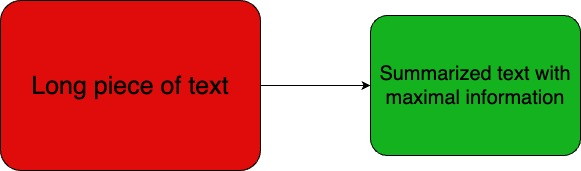
\includegraphics[width=.8\textwidth]{images/summarize.jpg}
  \end{figure}

\end{frame}


\subsection{Automatic Summarization}

\begin{frame}{What's Automatic Summarization?}

  Summarization done by a computer algorithm automatically is known as automatic
  summarization.

  \vskip .5cm

  \begin{itemize}
    \item \textbf{Extractive methods} extract key sentences or phrases from the text.
    \item \textbf{Abstractive methods} generate summary from scratch. Higher quality of summaries than extractive methods but are computationally expensive.
  \end{itemize}

  \vskip .5cm

  \begin{figure}
    \centering
    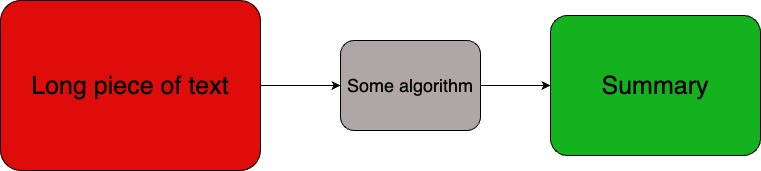
\includegraphics[width=.9\textwidth]{images/algorithm-summarize.jpg}
  \end{figure}

\end{frame}

\begin{frame}{How is it done today?}

  Nowadays, we have sophisticated Large Language Models (LLMs) based on the Transformer architecture \citep{vaswani2017attention} for automatic summarization.
  These methods have pushed the boundaries of abstractive summarization and can generate accurate, coherent, and human-like summaries.

  \vskip 1.3cm

  \begin{figure}
    \centering
    
\includegraphics[width=.25\textwidth]{images/GPT-4.png}
    \hskip 1cm
    
\includegraphics[width=.45\textwidth]{images/llama.jpg}
  \end{figure}

\end{frame}
